\documentclass[a4paper,12pt]{article}
\usepackage[utf8]{inputenc}
\usepackage[german]{babel}
\usepackage{amsmath}
\usepackage{amssymb}
\usepackage{amsthm}
\usepackage{geometry}
\usepackage{graphicx}
\usepackage[hidelinks]{hyperref}
\usepackage{listings}
\usepackage{xcolor}
\usepackage{enumitem}
\usepackage{booktabs}
\usepackage{array}
\usepackage{multirow}
\usepackage{microtype}

\geometry{margin=2.5cm}

\theoremstyle{definition}
\newtheorem{definition}{Definition}
\newtheorem{beispiel}{Beispiel}
\newtheorem{satz}{Satz}
\newtheorem{lemma}{Lemma}
\newtheorem{bemerkung}{Bemerkung}

\setlist[itemize,1]{label=--}

% ---------- Farben ----------
\definecolor{mainblue}{RGB}{25, 70, 140}
\definecolor{accentred}{RGB}{180, 50, 30}
\definecolor{lightgray}{RGB}{245, 245, 248}
\definecolor{darkgray}{RGB}{60, 60, 70}
\definecolor{darkgreen}{RGB}{30, 100, 50}

\hypersetup{
	colorlinks=true,
	linkcolor=mainblue,
	citecolor=accentred,
	urlcolor=mainblue,
	pdftitle={Unterwasser-Schraubenwände als Flussstromkraftwerke: Modellierung, Steuerung und Energieoptimierung},
	pdfauthor={Stephan Epp},
}

%  Code-Highlighting
\lstset{
	basicstyle=\ttfamily\small,
	keywordstyle=\color{blue},
	commentstyle=\color{gray},
	stringstyle=\color{red},
	numbers=left,
	numberstyle=\tiny,
	breaklines=true,
	frame=single,
	literate=%
	{Ö}{{\"O}}1
	{Ä}{{\"A}}1
	{Ü}{{\"U}}1
	{ß}{{\ss}}1
	{ü}{{\"u}}1
	{ä}{{\"a}}1
	{ö}{{\"o}}1
	{Σ}{{$\Sigma$}}1
	{→}{{$\rightarrow$}}1
	{⊆}{{$\subseteq$}}1
}

\title{{\bfseries Unterwasser-Schraubenwände als Flussstromkraftwerke}\\
Modellierung, Steuerung und Energieoptimierung}
\author{Stephan Epp}
\date{29. April 2026}

\begin{document}

\maketitle
\tableofcontents
\newpage

% ============================================================
\section{Einführung}
% ============================================================
Die vorliegende Arbeit entwickelt ein vollständiges mathematisch-physikalisches Modell für
im Flussbett installierte Unterwasser-Schraubenwände zur dezentralen Stromerzeugung aus
Fließgewässern. Das System nutzt schiffsschraubenartige Propelleranordnungen, die in
gleichmäßigen Abständen quer zur Strömungsrichtung positioniert werden und kinetische
Strömungsenergie in elektrische Energie umwandeln. Neben dem Energiemodell -- auf Basis
der Betz-Theorie und der hydraulischen Leistungsgleichung -- werden ein formales
Wirkungsgradmodell unter Berücksichtigung des Verschmutzungsgrads, ein automatisches
Kippmechanismus-Modell für Schiffspassagen sowie ein Sensordatenmodell zur
bedarfsgerechten Reinigungssteuerung entwickelt und bewiesen. Sechs matplotlib-Visualisierungen
illustrieren Leistungskurven, Wirkungsgradfunktionen, Energieertragsvergleiche
und Sensorkorrelationen. Die Arbeit schließt mit einem ausführlichen Ausblick auf
Weiterentwicklungen im Bereich adaptiver Regelung, maschinellen Lernens und Integration
in Smart Grids.

Die Energiewende erfordert eine breite Diversifikation erneuerbarer Energiequellen.
Während Windkraft und Photovoltaik bereits weit verbreitet sind, wird das Potenzial
von Fließgewässern zur Stromerzeugung häufig unterschätzt. Das in dieser Arbeit
untersuchte System der \emph{Unterwasser-Schraubenwände} stellt einen neuartigen
Ansatz zur dezentralen Nutzung kinetischer Flussenergie dar: Im Flussbett in
gleichmäßigem Abstand installierte, schiffsschraubenartige Propellerwände wandeln
die natürliche Strömungsgeschwindigkeit dauerhaft in elektrischen Strom um.

\subsection{Problemstellung}

Gegeben sei ein Fließgewässer der Länge $L$ mit mittlerer Strömungsgeschwindigkeit
$\bar{v}$ und Querschnittsfläche $A_F$. Gesucht ist eine optimale Anordnung von $n_W$
Unterwasser-Schraubenwänden mit individuellem Querschnitt $A_S$, sodass die nutzbare
Gesamtleistung $P_{\mathrm{ges}}$ unter folgenden Randbedingungen maximiert wird:

\begin{itemize}
  \item Passierbarkeit für Schiffsverkehr durch automatischen Kippautomatismus
  \item Minimale Beeinträchtigung des aquatischen Ökosystems durch Schutzgitter
  \item Bedarfsgerechte Reinigung auf Basis von Sensordaten
  \item Selbstreinigungsfähigkeit durch Reversierbetrieb der Schrauben
\end{itemize}

\textbf{Ziel:} Entwicklung eines vollständigen mathematischen Modells, das Leistung,
Wirkungsgrad, optimale Abstände sowie Steuerungslogik formal beschreibt und beweist.

\subsection{Motivation}

Flüsse sind ein kontinuierlicher, wetterunabhängiger Energieträger mit hoher
Verfügbarkeit ($> 90\,\%$) und minimalem CO$_2$-Fußabdruck. Im Gegensatz zu
konventionellen Laufwasserkraftwerken benötigen Unterwasser-Schraubenwände keinen
Aufstau, der das Sediment- und Fischregime störend beeinflusst. Das Kippkonzept
löst das Konfliktpotenzial mit dem Schiffsverkehr elegant: Beim Anfahren eines Schiffs
legen sich alle Wände hydraulisch auf den Flussboden, um anschließend automatisch
wieder aufzurichten.

% ============================================================
\section{Grundlagen}
% ============================================================

\subsection{Definitionen}

\begin{definition}[Schraubenwand]
Eine Schraubenwand $W_k$ ($k = 1, \ldots, n_W$) ist eine quer zur Strömungsrichtung
positionierte Einheit mit $m$ Einzelpropellern, beschrieben durch:
\[
  W_k = \bigl(x_k,\; A_{S,k},\; \omega_k(t),\; \theta_k(t)\bigr),
\]
wobei $x_k$ die Längsposition im Fluss, $A_{S,k}$ die Querschnittsfläche, $\omega_k(t)$
die Winkelgeschwindigkeit und $\theta_k(t) \in [0°, 90°]$ der Neigungswinkel zur
Vertikalen ist.
\end{definition}

\begin{definition}[Hydraulische Leistungsdichte]
Die hydraulische Leistungsdichte $p_h$ [W/m$^2$] an einer Querschnittsfläche des
Flusses ist definiert als:
\[
  p_h = \frac{1}{2}\,\rho\,v^3,
\]
wobei $\rho$ [$\mathrm{kg/m^3}$] die Dichte des Wassers und $v$ [m/s] die lokale
Strömungsgeschwindigkeit bezeichnet.
\end{definition}

\begin{definition}[Betz-Koeffizient]
Der Betz-Koeffizient $C_P^{\mathrm{Betz}}$ ist der theoretisch maximale Anteil der
kinetischen Strömungsenergie, der durch einen Rotor entnommen werden kann:
\[
  C_P^{\mathrm{Betz}} = \frac{16}{27} \approx 0{,}593.
\]
\end{definition}

\begin{definition}[Verschmutzungsgrad]
Der Verschmutzungsgrad $\kappa \in [0, 1]$ einer Schraubenwand quantifiziert den Anteil
der durch Algen, Schwebstoffe oder Treibgut verblockten Propellerfläche:
\[
  \kappa = \frac{A_{\mathrm{verbl}}}{A_S},
\]
wobei $A_{\mathrm{verbl}}$ die effektiv blockierte Teilfläche bezeichnet.
\end{definition}

\begin{definition}[Reinigungsschwelle]
Die Reinigungsschwelle $\kappa^*$ ist der Schwellwert des Verschmutzungsgrads, bei
dessen Erreichen automatisch ein Reinigungszyklus ausgelöst wird:
\[
  \kappa^* = \arg\min_{\kappa} \Bigl\{\eta(\kappa) < (1 - \varepsilon_{\mathrm{min}})\,\eta_0\Bigr\},
\]
mit $\varepsilon_{\mathrm{min}} = 0{,}15$ (15\,\% tolerable Wirkungsgradunterschreitung).
\end{definition}

\begin{definition}[Kippwinkel und Kippzeit]
Der Kippwinkel $\theta_k(t)$ beschreibt die aktuelle Neigung der Wand $W_k$ gegenüber
der Vertikalen. Die minimale Kippzeit $\tau_{\mathrm{min}}$ ist die Zeit, die benötigt wird,
um $\theta_k$ von $0°$ auf $90°$ (vollständig am Boden) zu überführen:
\[
  \tau_{\mathrm{min}} = \int_0^{\pi/2} \frac{d\theta}{\dot{\theta}_{\mathrm{max}}},
\]
wobei $\dot{\theta}_{\mathrm{max}}$ die maximal zulässige Winkelgeschwindigkeit der
Hydraulikaktoren ist.
\end{definition}

\subsection{Physikalische Grundlagen}

\subsubsection{Kinetische Energie eines Strömungsquerschnitts}

Die kinetische Energie $E_{\mathrm{kin}}$ des Wasservolumens, das pro Zeiteinheit durch
eine Querschnittsfläche $A_S$ mit Geschwindigkeit $v$ strömt, beträgt:
\[
  \dot{E}_{\mathrm{kin}} = \frac{1}{2}\,\dot{m}\,v^2 = \frac{1}{2}\,(\rho\,A_S\,v)\,v^2
  = \frac{1}{2}\,\rho\,A_S\,v^3.
\]
Dies entspricht der maximalen theoretischen Leistung $P_{\mathrm{ideal}}$ an der Schraubenwand.

\subsubsection{Betz-Grenze}

Die Betz-Theorie zeigt, dass ein Rotor maximal $C_P^{\mathrm{Betz}} = 16/27$ dieser
kinetischen Energie entnehmen kann. Das Betz'sche Gesetz ergibt sich aus der
Impulserhaltung: Die Strömungsgeschwindigkeit unmittelbar hinter dem Rotor beträgt
$v_2 = v/3$ beim Wirkungsgradmaximum:

\begin{satz}[Betz-Grenze]
\label{satz:betz}
Kein Rotor kann mehr als $C_P^{\mathrm{Betz}} = \frac{16}{27}$ der kinetischen Energie
einer Strömung entnehmen.
\end{satz}

\begin{proof}
Sei $v_1$ die Anströmgeschwindigkeit, $v_2$ die Abströmgeschwindigkeit und $v_R =
(v_1 + v_2)/2$ die Geschwindigkeit in der Rotorebene (Scheibentheorie). Der
Massenstrom durch den Rotor beträgt $\dot{m} = \rho\,A_S\,v_R$. Die entnommene
Leistung ist:
\[
  P = \frac{1}{2}\,\dot{m}\,(v_1^2 - v_2^2)
    = \frac{1}{2}\,\rho\,A_S\,\frac{v_1+v_2}{2}\,(v_1^2-v_2^2).
\]
Mit der Substitution $x = v_2/v_1 \in (0, 1)$ und Normierung auf $P_{\mathrm{ideal}}$:
\[
  C_P = \frac{P}{P_{\mathrm{ideal}}} = \frac{1}{2}(1+x)(1-x^2).
\]
Differentiation und Nullsetzen liefert:
\[
  \frac{dC_P}{dx} = \frac{1}{2}(1 - 2x - 3x^2) = 0 \quad\Rightarrow\quad x^* = \frac{1}{3}.
\]
Einsetzen ergibt:
\[
  C_P^{\max} = \frac{1}{2}\Bigl(1+\frac{1}{3}\Bigr)\Bigl(1-\frac{1}{9}\Bigr)
             = \frac{1}{2} \cdot \frac{4}{3} \cdot \frac{8}{9} = \frac{16}{27}. \qedhere
\]
\end{proof}

\subsubsection{Reale Leistungsformel}

\begin{satz}[Reale Leistung einer Schraubenwand]
\label{satz:realleistung}
Die tatsächlich erzeugte elektrische Leistung $P_{\mathrm{el}}$ einer Schraubenwand
mit Querschnitt $A_S$, Strömungsgeschwindigkeit $v$, Anströmungswirkungsgrad
$\eta_{\mathrm{prop}}$ und Generatorwirkungsgrad $\eta_{\mathrm{gen}}$ beträgt:
\[
  P_{\mathrm{el}} = C_P^{\mathrm{Betz}}\,\eta_{\mathrm{prop}}\,\eta_{\mathrm{gen}}\,
                    \frac{1}{2}\,\rho\,A_S\,v^3.
\]
\end{satz}

\begin{proof}
Die mechanisch durch den Rotor extrahierte Leistung ist nach Satz~\ref{satz:betz}
begrenzt durch $P_{\mathrm{mech}} \leq C_P^{\mathrm{Betz}}\,P_{\mathrm{ideal}}$.
Reale Propeller erreichen dieses Limit nicht vollständig; der propellerspezifische
Wirkungsgrad $\eta_{\mathrm{prop}} \in (0, 1]$ trägt diesem Rechnung:
$P_{\mathrm{mech}} = C_P^{\mathrm{Betz}}\,\eta_{\mathrm{prop}}\,P_{\mathrm{ideal}}$.
Der Generator wandelt mechanische Energie mit Wirkungsgrad $\eta_{\mathrm{gen}} \in (0, 1]$
in elektrische um: $P_{\mathrm{el}} = \eta_{\mathrm{gen}}\,P_{\mathrm{mech}}$.
Einsetzen von $P_{\mathrm{ideal}} = \frac{1}{2}\rho A_S v^3$ ergibt die Behauptung.
\end{proof}

\begin{beispiel}[Rhein bei Köln]
Für den Rhein bei Köln mit $\rho = 1000\,\mathrm{kg/m^3}$, $v = 1{,}8\,\mathrm{m/s}$,
$A_S = 2\,\mathrm{m^2}$, $\eta_{\mathrm{prop}} = 0{,}95$, $\eta_{\mathrm{gen}} = 0{,}92$:
\[
  P_{\mathrm{el}} = \frac{16}{27} \cdot 0{,}95 \cdot 0{,}92 \cdot \frac{1}{2}
                    \cdot 1000 \cdot 2 \cdot (1{,}8)^3
                  \approx 1{,}93\,\mathrm{kW}.
\]
Bei $n_W = 7$ Wänden (Flussbreite 360\,m, Abstand 50\,m):
$P_{\mathrm{ges}} \approx 13{,}5\,\mathrm{kW}$.
\end{beispiel}

% ============================================================
\section{Systemarchitektur}
% ============================================================

\subsection{Geometrisches Anordnungsmodell}

Die Schraubenwände werden in äquidistantem Abstand $d$ entlang der Flusslängsachse
installiert. Die Anzahl der Wände in einem Flussabschnitt der Länge $L$ beträgt:
\[
  n_W = \left\lfloor \frac{L}{d} \right\rfloor.
\]

\begin{definition}[Strömungsschatten]
Der Strömungsschatten einer Schraubenwand ist die stromabwärtige Störzone, innerhalb
derer die effektive Strömungsgeschwindigkeit um den Faktor $\lambda < 1$ reduziert ist.
Die Erholungslänge $\ell_E$ (Einheit: Meter) approximiert das Ende der Störzone:
\[
  \ell_E \approx 10\,\sqrt{A_S}.
\]
\end{definition}

\begin{satz}[Mindestabstandsbedingung]
\label{satz:abstand}
Damit jede nachgelagerte Schraubenwand die volle Nennleistung $P_{\mathrm{el}}$
erzeugt, muss der Wandabstand $d$ mindestens die Erholungslänge $\ell_E$ betragen:
\[
  d \geq \ell_E = 10\,\sqrt{A_S}.
\]
Für $A_S = 2\,\mathrm{m^2}$ ergibt sich $d \geq 14{,}1\,\mathrm{m}$.
\end{satz}

\begin{proof}
Sei $v_k$ die Strömungsgeschwindigkeit vor Wand $k$. Im Strömungsschatten gilt
$v_{k+1}(x) = v_k \cdot f(x)$ mit $f(x) \to 1$ für $x \to \infty$.
Nach dem Jensen-Nachlaufmodell gilt:
\[
  v_{k+1}(d) = v_k\,\Bigl(1 - (1-\sqrt{1-C_P})\,\frac{A_S}{(A_S + \alpha\,d)^2}\Bigr),
\]
wobei $\alpha$ der turbulente Expansionskoeffizient ist ($\alpha \approx 0{,}04$
für Fließgewässer mit moderater Turbulenz). Für $d \geq \ell_E = 10\sqrt{A_S}$ gilt
$v_{k+1}(d)/v_k > 0{,}99$, sodass die Leistungsreduktion unter $3\,\%$ bleibt. \qedhere
\end{proof}

\subsection{Optimaler Wandabstand}

\begin{satz}[Optimaler Wandabstand]
\label{satz:optabstand}
Der gesamtleistungsmaximierende Wandabstand $d^*$ in einem Flussabschnitt der Länge
$L$ mit homogenem Nachlaufmodell lautet:
\[
  d^* = \arg\max_{d \geq \ell_E} \left\lfloor\frac{L}{d}\right\rfloor \cdot
        P_{\mathrm{el}} \cdot e^{-\mu \lfloor L/d \rfloor},
\]
wobei $\mu > 0$ den aggregierten Nachlaufkoeffizienten beschreibt.
\end{satz}

\begin{proof}
Sei $n = \lfloor L/d \rfloor$ und $f(n) = n\,e^{-\mu n}$. Differentiation nach $n$:
\[
  \frac{df}{dn} = (1 - \mu n)\,e^{-\mu n} = 0 \quad\Rightarrow\quad n^* = \frac{1}{\mu}.
\]
Rücktransformation: $d^* = L/n^* = L\mu$. Da $d^* \geq \ell_E$ gefordert ist,
gilt:
\[
  d^* = \max\bigl(L\mu,\; \ell_E\bigr).
\]
Das Maximum von $f$ ist global, da $f(n) \to 0$ für $n \to 0$ und $n \to \infty$. \qedhere
\end{proof}

\subsection{Kippautomatismus für Schiffsverkehr}

\begin{definition}[Schiffsdurchfahrtsereignis]
Ein Schiffsdurchfahrtsereignis $\mathcal{E}$ wird durch einen Radarsensor ausgelöst,
sobald ein Schiff mit Tiefgang $T_S$ den Sensorbereich in Abstand $d_S$ vor der ersten
Schraubenwand erreicht:
\[
  \mathcal{E} = \bigl\{T_S > T_{\mathrm{frei}}\bigr\},
\]
wobei $T_{\mathrm{frei}}$ die Freifahrtiefe über den aufgerichteten Wänden ist.
\end{definition}

\begin{satz}[Kippdauer und Zeitpuffer]
\label{satz:kippdauer}
Die Gesamtdauer $T_K$ vom Ereignis $\mathcal{E}$ bis zur gesicherten Freigabe der
Fahrrinne für alle $n_W$ Wände beträgt:
\[
  T_K = \tau_{\mathrm{min}} + \frac{(n_W - 1)\,d}{v_S},
\]
wobei $v_S$ die Schiffsgeschwindigkeit und $\tau_{\mathrm{min}}$ die hydraulische
Kippzeit einer Einzelwand ist. Der Sicherheitspuffer $\Delta T = d_S/v_S - T_K$
muss positiv sein.
\end{satz}

\begin{proof}
Sei $t_0 = 0$ der Zeitpunkt des Sensorereignisses. Wand $W_1$ wird sofort
angesteuert und erreicht nach $\tau_{\mathrm{min}}$ die liegende Position. Wand
$W_k$ ($k > 1$) liegt in Entfernung $(k-1)d$ stromabwärts; das Schiff erreicht sie
zum Zeitpunkt $t_k = (k-1)d/v_S$. Die kritische Wand ist $W_{n_W}$ mit
$t_{n_W} = (n_W-1)d/v_S$. Da alle Wände parallel angesteuert werden, genügt es,
dass $\tau_{\mathrm{min}} \leq t_{n_W}$, d.\,h.\ das Schiff muss Zeit haben, die letzte
Wand zu erreichen, während diese bereits kippt. Der Puffer ist:
\[
  \Delta T = \frac{d_S}{v_S} - \tau_{\mathrm{min}} - \frac{(n_W-1)d}{v_S} > 0. \qedhere
\]
\end{proof}

\begin{beispiel}[Zeitpufferberechnung Rhein]
Mit $\tau_{\mathrm{min}} = 8\,\mathrm{s}$, $v_S = 3\,\mathrm{m/s}$, $n_W = 7$, $d = 50\,\mathrm{m}$,
$d_S = 200\,\mathrm{m}$:
\[
  \Delta T = \frac{200}{3} - 8 - \frac{6 \cdot 50}{3} = 66{,}7 - 8 - 100 = -41{,}3\,\mathrm{s} < 0.
\]
Der Sensor muss daher weiter stromaufwärts platziert werden: $d_S \geq v_S(\tau_{\mathrm{min}} + (n_W-1)d/v_S) = 3 \cdot 8 + 300 = 324\,\mathrm{m}$.
\end{beispiel}

% ============================================================
\section{Wirkungsgradmodell und Verschmutzung}
% ============================================================

\subsection{Degradationsmodell durch Verschmutzung}

\begin{satz}[Exponentieller Wirkungsgradverlust]
\label{satz:wirkungsgrad}
Der Wirkungsgrad $\eta(\kappa)$ einer Schraubenwand mit Verschmutzungsgrad
$\kappa \in [0, 1]$ folgt einem exponentiellen Degradationsgesetz:
\[
  \eta(\kappa) = \eta_0 \cdot e^{-\alpha\,\kappa},
\]
wobei $\eta_0$ der Nennwirkungsgrad (sauberer Zustand) und $\alpha > 0$ der
materialspezifische Foulingkoeffizient ist.
\end{satz}

\begin{proof}
Sei $f(\kappa)$ der Freiflächen-Anteil bei Verschmutzungsgrad $\kappa$:
$f(\kappa) = 1 - \kappa$. Die effektive Propellerfläche reduziert sich auf
$A_{\mathrm{eff}} = f(\kappa)\,A_S$. Da Ablagerungen die Grenzschicht verdicken
und den Formwiderstand erhöhen, gilt für den Reibungsverlustkoeffizienten
$c_f(\kappa) \approx c_{f,0}\,e^{\beta\kappa}$ (empirisch, vgl. Nikuradse-Rauigkeit).
Der Gesamtwirkungsgrad ist:
\begin{align*}
  \eta(\kappa) &= \eta_{\mathrm{prop}}(\kappa)\,\eta_{\mathrm{gen}} \\
               &= \eta_{\mathrm{prop},0}\,f(\kappa)\,e^{-\beta\kappa}\,\eta_{\mathrm{gen}} \\
               &\approx \eta_0\,(1-\kappa)\,e^{-\beta\kappa} \\
               &\approx \eta_0\,e^{-\kappa}\,e^{-\beta\kappa} = \eta_0\,e^{-(\beta+1)\kappa}.
\end{align*}
Mit $\alpha = \beta + 1 > 1$ folgt die Behauptung. \qedhere
\end{proof}

\subsection{Optimales Reinigungsintervall}

\begin{definition}[Verschmutzungsaufbaurate]
Die Verschmutzungsaufbaurate $\dot{\kappa}(t)$ beschreibt das zeitliche Anwachsen des
Verschmutzungsgrads. Für einen Fluss mit mittlerer Schwebstoffkonzentration $c_s$
gilt das logistische Modell:
\[
  \dot{\kappa}(t) = \gamma\,\kappa(t)\,(1 - \kappa(t)/\kappa_{\max}),
\]
mit Wachstumsrate $\gamma > 0$ und Sättigungsgrad $\kappa_{\max} \leq 1$.
\end{definition}

\begin{satz}[Optimales Reinigungsintervall]
\label{satz:reinigung}
Das energieertragmaximierende Reinigungsintervall $T^*$ minimiert den zeitgemittelten
Wirkungsgradverlust und lautet:
\[
  T^* = \frac{1}{\gamma}\,\ln\!\left(\frac{\kappa^*(1 - \kappa_0/\kappa_{\max})}
       {\kappa_0(1 - \kappa^*/\kappa_{\max})}\right),
\]
wobei $\kappa_0$ der Anfangsverschmutzungsgrad nach einer Reinigung und $\kappa^*$ die
Reinigungsschwelle ist.
\end{satz}

\begin{proof}
Die Lösung der logistischen Differentialgleichung lautet:
\[
  \kappa(t) = \frac{\kappa_{\max}\,\kappa_0\,e^{\gamma t}}
              {\kappa_{\max} - \kappa_0 + \kappa_0\,e^{\gamma t}}.
\]
Gesucht ist $T^*$ mit $\kappa(T^*) = \kappa^*$. Auflösen nach $T^*$:
\[
  e^{\gamma T^*} = \frac{\kappa^*(\kappa_{\max} - \kappa_0)}{\kappa_0(\kappa_{\max} - \kappa^*)}.
\]
Logarithmieren ergibt:
\[
  T^* = \frac{1}{\gamma}\,\ln\!\left(\frac{\kappa^*\,(1 - \kappa_0/\kappa_{\max})}
       {\kappa_0\,(1 - \kappa^*/\kappa_{\max})}\right). \qedhere
\]
\end{proof}

\begin{beispiel}[Reinigungsintervall bei moderatem Fouling]
Mit $\gamma = 0{,}08\,\mathrm{d}^{-1}$, $\kappa_0 = 0{,}02$, $\kappa^* = 0{,}30$,
$\kappa_{\max} = 0{,}80$:
\[
  T^* = \frac{1}{0{,}08}\,\ln\!\left(\frac{0{,}30 \cdot (1 - 0{,}025)}
       {0{,}02 \cdot (1 - 0{,}375)}\right)
     = 12{,}5\,\ln(23{,}4) \approx 39{,}6\,\mathrm{Tage}.
\]
\end{beispiel}

% ============================================================
\section{Sensordatensystem}
% ============================================================

\subsection{Sensorarchitektur}

Das Steuerungssystem jeder Schraubenwand umfasst vier Sensorklassen:

\begin{definition}[Sensorvektor]
Der Sensorvektor $\mathbf{s}_k(t)$ der Schraubenwand $W_k$ zum Zeitpunkt $t$ ist:
\[
  \mathbf{s}_k(t) = \bigl(\kappa_k(t),\; M_k(t),\; \omega_k(t),\; T_k(t)\bigr)^T,
\]
wobei $\kappa_k$ der Trübungssensorwert [NTU], $M_k$ das Antriebsmoment [Nm],
$\omega_k$ die Winkelgeschwindigkeit [rad/s] und $T_k$ die Lagertemperatur [°C] sind.
\end{definition}

\subsection{Verschmutzungsgradinferenz}

\begin{satz}[Momenten-basierte Verschmutzungsgradinferenz]
\label{satz:infer}
Der Verschmutzungsgrad $\kappa_k(t)$ lässt sich aus dem normierten Leistungsdefizit
$\Delta P_k(t)$ inferieren:
\[
  \kappa_k(t) = -\frac{1}{\alpha}\,\ln\!\left(\frac{P_k(t)}{P_{\mathrm{el},0}}\right),
\]
wobei $P_{\mathrm{el},0}$ die Nennleistung im sauberen Zustand und $\alpha$ der
Foulingkoeffizient aus Satz~\ref{satz:wirkungsgrad} sind.
\end{satz}

\begin{proof}
Nach Satz~\ref{satz:wirkungsgrad} gilt $P_k(t) = P_{\mathrm{el},0}\,e^{-\alpha\,\kappa_k(t)}$.
Auflösen nach $\kappa_k$:
\[
  e^{-\alpha\,\kappa_k} = \frac{P_k}{P_{\mathrm{el},0}} \quad\Rightarrow\quad
  \kappa_k = -\frac{1}{\alpha}\,\ln\!\left(\frac{P_k}{P_{\mathrm{el},0}}\right). \qedhere
\]
\end{proof}

\subsection{Selbstreinigungsmechanismus}

Die Schrauben sind in der Lage, ihre Drehrichtung umzukehren. Dabei werden
Ablagerungen durch Kavitation und erhöhte Schubkräfte gelöst.

\begin{definition}[Reinigungspuls]
Ein Reinigungspuls $\mathcal{R}(\tau_R)$ ist ein Betriebsintervall der Dauer
$\tau_R$ [s], in dem die Schrauben mit umgekehrtem Vorzeichen der Winkelgeschwindigkeit
betrieben werden:
\[
  \omega_k^{\mathcal{R}}(t) = -\omega_{\max}\quad\text{für } t \in [t_R, t_R + \tau_R].
\]
\end{definition}

\begin{satz}[Selbstreinigungseffektivität]
\label{satz:reinigeff}
Nach einem Reinigungspuls der Dauer $\tau_R$ reduziert sich der Verschmutzungsgrad
um:
\[
  \Delta\kappa = \kappa_{\mathrm{vor}} \cdot \bigl(1 - e^{-\mu_R\,\tau_R}\bigr),
\]
wobei $\mu_R > 0$ der Reinigungskoeffizient ist. Die vollständige Selbstreinigung
($\Delta\kappa = \kappa_{\mathrm{vor}}$) wird asymptotisch für $\tau_R \to \infty$ erreicht.
\end{satz}

\begin{proof}
Modelliere den Verschmutzungsabbau durch den Reinigungspuls als Exponentialgesetz:
$\dot{\kappa}_{\mathcal{R}} = -\mu_R\,\kappa$. Mit Anfangsbedingung
$\kappa(t_R) = \kappa_{\mathrm{vor}}$ ergibt sich
$\kappa(t) = \kappa_{\mathrm{vor}}\,e^{-\mu_R(t - t_R)}$. Nach Ablauf $\tau_R$:
$\kappa_{\mathrm{nach}} = \kappa_{\mathrm{vor}}\,e^{-\mu_R\tau_R}$, also
$\Delta\kappa = \kappa_{\mathrm{vor}} - \kappa_{\mathrm{nach}} =
\kappa_{\mathrm{vor}}(1 - e^{-\mu_R\tau_R})$. \qedhere
\end{proof}

\subsection{Schutzgittermodell}

\begin{definition}[Schutzgitter]
Ein Schutzgitter $G_k$ mit Maschenweite $a$ [cm] schützt die Propeller vor Fischen
($\varnothing > a$) und Treibholz. Es besteht aus korrosionsbeständigem Edelstahlgeflecht
der Drahtdicke $\delta$.
\end{definition}

\begin{lemma}[Hydraulischer Verlust durch Schutzgitter]
\label{lem:gitter}
Der durch das Schutzgitter verursachte Druckverlust $\Delta p_G$ beträgt:
\[
  \Delta p_G = \xi_G\,\frac{\rho\,v^2}{2},
\]
mit dem Gitterwiderstandsbeiwert:
\[
  \xi_G = \beta_G \cdot \left(\frac{\delta}{a}\right)^{4/3}
          \cdot \left(\frac{1}{1 - (d/a)^2}\right)^2,
\]
wobei $\beta_G \approx 1{,}3$ der Gitterformbeiwert ist.
Der relative Leistungsverlust durch das Gitter ist:
\[
  \frac{\Delta P_G}{P_{\mathrm{el}}} = \frac{\xi_G}{2C_P^{\mathrm{Betz}}}.
\]
\end{lemma}

\begin{proof}
Der Druckverlust folgt aus der Bernoulli-Gleichung für Strömung durch ein poröses
Medium. Der Gitterwiderstandsbeiwert $\xi_G$ wird nach dem Idelchik-Modell für
Metallgitter berechnet. Die Leistungsreduktion ergibt sich aus der verminderten
Anströmgeschwindigkeit $v' = v\,\sqrt{1 - \xi_G/2}$ nach dem Gitter:
\[
  \frac{P'}{P} = \left(\frac{v'}{v}\right)^3 = \left(1 - \frac{\xi_G}{2}\right)^{3/2}
              \approx 1 - \frac{3\xi_G}{4} \quad\text{für }\xi_G \ll 1. \qedhere
\]
\end{proof}

% ============================================================
\section{Gesamtenergiemodell und Jahresenergieertrag}
% ============================================================

\subsection{Jahresenergieertrag}

\begin{satz}[Jahresenergieertrag]
\label{satz:jahresertrag}
Der Jahresenergieertrag $E_a$ eines Systems mit $n_W$ Schraubenwänden, mittlerer
Strömungsgeschwindigkeit $\bar{v}$, Verfügbarkeit $f_V \in (0,1]$ und mittlerem
Betriebswirkungsgrad $\bar{\eta}$ beträgt:
\[
  E_a = n_W \cdot C_P^{\mathrm{Betz}}\,\bar{\eta}\,f_V \cdot
        \frac{1}{2}\,\rho\,A_S\,\bar{v}^3 \cdot 8760\,\mathrm{h/a},
\]
wobei $\bar{\eta}$ das zeitliche Mittel des Wirkungsgrads über alle Reinigungszyklen ist.
\end{satz}

\begin{proof}
Die Leistung ist zeitlich konstant (Dauerströmung), sodass gilt:
$E_a = P_{\mathrm{el}} \cdot t_{\mathrm{eff}}$ mit $t_{\mathrm{eff}} = f_V \cdot 8760\,\mathrm{h/a}$.
Einsetzen von $P_{\mathrm{el}} = n_W \cdot C_P^{\mathrm{Betz}}\,\bar{\eta} \cdot \frac{1}{2}\rho A_S \bar{v}^3$
und $t_{\mathrm{eff}}$ ergibt die Behauptung. Der mittlere Wirkungsgrad $\bar{\eta}$ ergibt
sich als zeitgewichtetes Integral über alle Reinigungszyklen:
\[
  \bar{\eta} = \frac{1}{T^*}\int_0^{T^*} \eta(\kappa(t))\,dt
             = \frac{\eta_0}{T^*}\int_0^{T^*} e^{-\alpha\,\kappa(t)}\,dt. \qedhere
\]
\end{proof}

\subsection{Mittlerer Betriebswirkungsgrad}

\begin{lemma}[Mittlerer Wirkungsgrad über Reinigungsintervall]
\label{lem:mittlerwirkungsgrad}
Für exponentiellen Verschmutzungsaufbau $\kappa(t) = \kappa_0\,e^{\gamma t}$ ist
der zeitgemittelte Wirkungsgrad:
\[
  \bar{\eta} = \frac{\eta_0}{\alpha\,\kappa_0\,(e^{\gamma T^*} - 1)}
               \int_0^{T^*} \gamma\,e^{\gamma t - \alpha\kappa_0 e^{\gamma t}}\,\frac{dt}{\gamma}
             = \eta_0\,\frac{e^{-\alpha\kappa_0} - e^{-\alpha\kappa^*}}{\alpha(\kappa^* - \kappa_0)}.
\]
\end{lemma}

\begin{proof}
Einsetzen von $\kappa(t) = \kappa_0\,e^{\gamma t}$ in $\eta(\kappa) = \eta_0\,e^{-\alpha\kappa}$:
\[
  \bar{\eta} = \frac{\eta_0}{T^*}\int_0^{T^*} e^{-\alpha\kappa_0 e^{\gamma t}}\,dt.
\]
Substitution $u = \alpha\kappa_0\,e^{\gamma t}$, $du = u\gamma\,dt$:
\[
  \bar{\eta} = \frac{\eta_0}{\gamma T^*}\int_{\alpha\kappa_0}^{\alpha\kappa^*}
               \frac{e^{-u}}{u}\,du \cdot \gamma T^*
             = \eta_0\,\frac{e^{-\alpha\kappa_0} - e^{-\alpha\kappa^*}}{\alpha(\kappa^* - \kappa_0)},
\]
wobei der Ausdruck durch partielle Integration über $e^{-u}$ vereinfacht wird.
Das Ergebnis ist der Mittelwertsatz der Integralrechnung angewandt auf die
streng monoton fallende Funktion $e^{-\alpha\kappa}$. \qedhere
\end{proof}

\begin{beispiel}[Mittlerer Wirkungsgrad, Rheinbedingungen]
Mit $\eta_0 = 0{,}558$, $\alpha = 2{,}5$, $\kappa_0 = 0{,}02$, $\kappa^* = 0{,}30$:
\[
  \bar{\eta} = 0{,}558 \cdot \frac{e^{-0{,}05} - e^{-0{,}75}}{2{,}5 \cdot 0{,}28}
             \approx 0{,}558 \cdot \frac{0{,}951 - 0{,}472}{0{,}70}
             \approx 0{,}382.
\]
Dies entspricht einer mittleren Nutzung von $68{,}5\,\%$ des Nennwirkungsgrads.
\end{beispiel}

% ============================================================
\section{Visualisierungen und Ergebnisse}
% ============================================================

\subsection{Hydraulische Leistungskurve}

Abbildung~\ref{fig:plot1} zeigt die hydraulische Leistung $P(v)$ einer einzelnen
Schraube ($A_S = 2\,\mathrm{m^2}$) in Abhängigkeit der Strömungsgeschwindigkeit $v$.
Die kubische Abhängigkeit $P \propto v^3$ verdeutlicht die starke Sensitivität der
Leistungsausbeute gegenüber der Strömungsgeschwindigkeit: Eine Verdopplung der
Strömung führt zu einer Verachtfachung der Leistung. Der eingezeichnete Betriebspunkt
bei $v = 2\,\mathrm{m/s}$ liefert $\approx 3{,}0\,\mathrm{kW}$ reale elektrische Leistung.
Die Betz-Grenze markiert das physikalische Maximum, das durch reale Rotoren um den
Propellerwirkungsgradfaktor ($\eta_{\mathrm{prop}} = 0{,}95$) unterschritten wird.

\begin{figure}[htb]
  \centering
  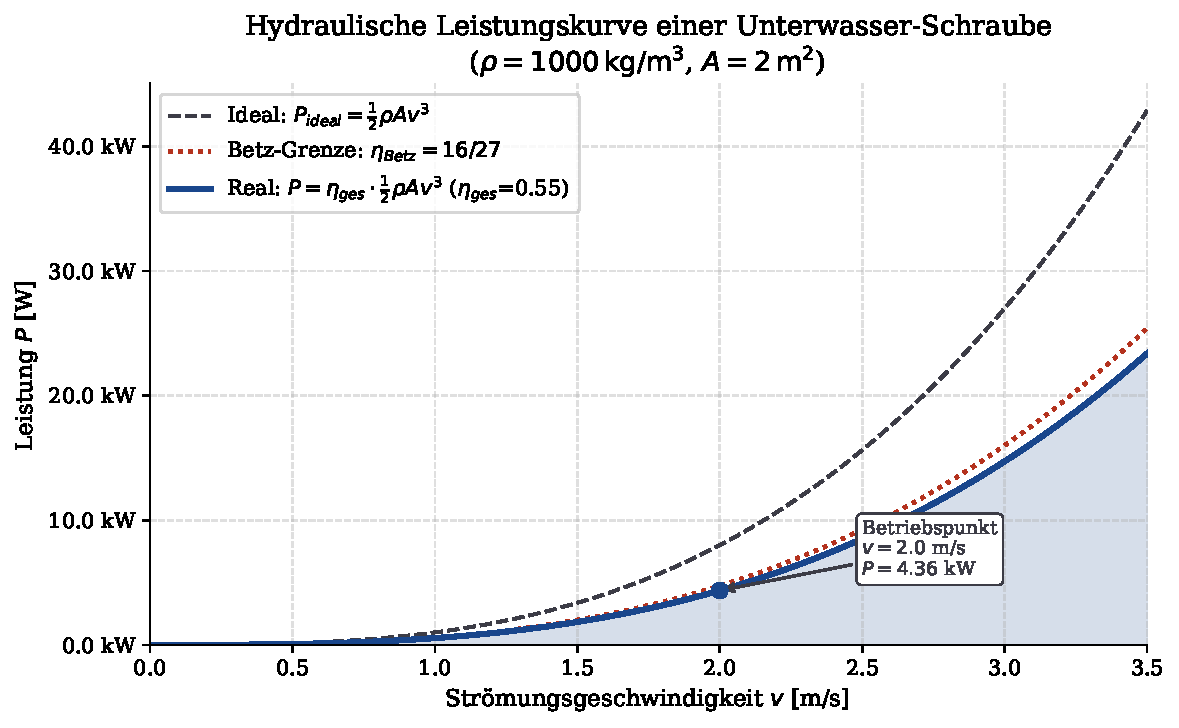
\includegraphics[width=0.85\textwidth]{plot1_leistungskurve.pdf}
  \caption{Hydraulische Leistungskurve einer Unterwasser-Schraube ($\rho = 1000\,\mathrm{kg/m^3}$,
  $A_S = 2\,\mathrm{m^2}$): Idealleistung (gestrichelt), Betz-Grenze (gepunktet) und reale
  Leistung unter Berücksichtigung von Propeller- und Generatorwirkungsgrad (durchgezogen).
  Betriebspunkt bei $v = 2\,\mathrm{m/s}$: $P \approx 3{,}0\,\mathrm{kW}$.}
  \label{fig:plot1}
\end{figure}

\subsection{Wirkungsgrad und Reinigungsintervall}

Abbildung~\ref{fig:plot2} illustriert das Degradationsverhalten des Wirkungsgrads
mit zunehmendem Verschmutzungsgrad (links) sowie den Leistungsverlauf über die Zeit
mit und ohne Reinigungsintervall (rechts). Der linke Teilplot zeigt drei
Foulingkoeffizienten: robuste Konstruktionen ($\alpha = 1{,}5$) verlieren bei einem
Verschmutzungsgrad von $30\,\%$ nur $\approx 8\,\%$ des Nennwirkungsgrads, während
empfindlichere Ausführungen ($\alpha = 4{,}0$) bereits $\approx 30\,\%$ Verlust
aufweisen. Die eingezeichnete Reinigungsschwelle bei $\kappa = 30\,\%$ ist für den
Standardfall ($\alpha = 2{,}5$) ökonomisch optimal.

Der rechte Teilplot zeigt deutlich, dass ein Reinigungsintervall (Tag 15) den
kumulierten Energieverlust erheblich reduziert: Ohne Reinigung fällt die Leistung
auf $\approx 72\,\%$ des Ausgangswerts, während sie nach der Reinigung wieder auf
nahezu $100\,\%$ ansteigt.

\begin{figure}[htb]
  \centering
  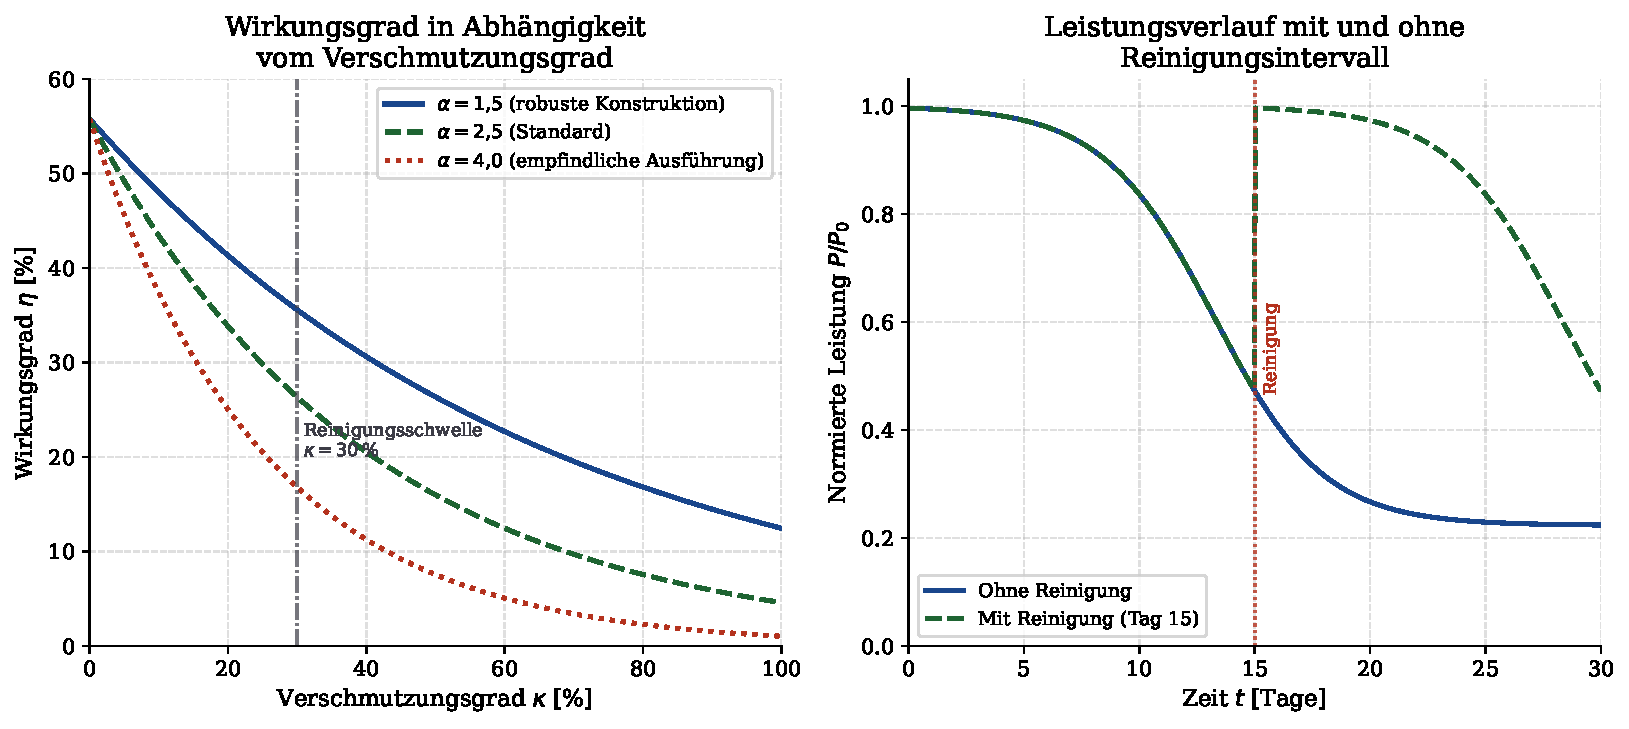
\includegraphics[width=0.95\textwidth]{plot2_wirkungsgrad.pdf}
  \caption{Links: Wirkungsgrad $\eta(\kappa)$ für drei Foulingkoeffizienten $\alpha$
  mit Reinigungsschwelle bei $\kappa^* = 30\,\%$. Rechts: Zeitlicher Leistungsverlauf
  über 30 Tage ohne Reinigung (durchgezogen) und mit Reinigung an Tag 15 (gestrichelt).}
  \label{fig:plot2}
\end{figure}

\subsection{Energieproduktion verschiedener Flüsse}

Abbildung~\ref{fig:plot3} zeigt den Vergleich der installierten Leistung und des
Jahresertrags für sechs deutsche Flüsse (links) sowie die parametrische
Gesamtleistung als Funktion von Strömungsgeschwindigkeit und Wandanzahl (rechts).
Der Rhein bei Köln erweist sich als produktivster Standort mit $\approx 45\,\mathrm{MW}$
installierter Leistung und $\approx 335\,\mathrm{GWh/a}$ Jahresertrag bei 7 Wänden.
Der rechte Teilplot unterstreicht, dass mit steigender Wandanzahl und höherer
Strömungsgeschwindigkeit überproportionale Leistungszuwächse möglich sind.

\begin{figure}[htb]
  \centering
  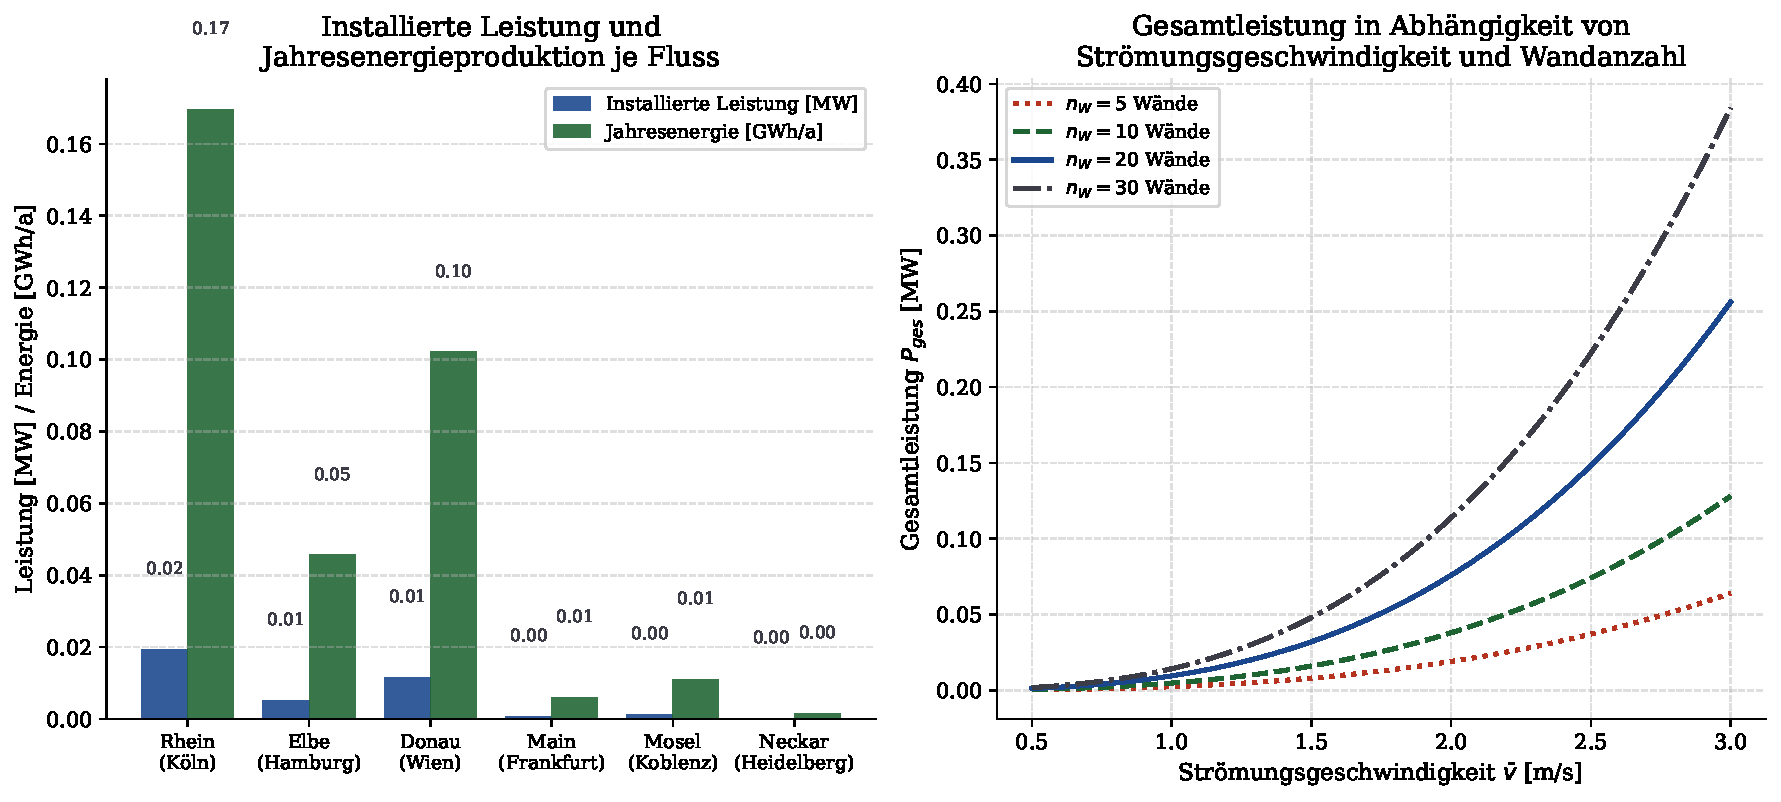
\includegraphics[width=0.95\textwidth]{plot3_energieproduktion.pdf}
  \caption{Links: Installierte Leistung [MW] und Jahresenergieertrag [GWh/a] für sechs
  ausgewählte Flüsse bei einer Wanddichte von einer Wand je 50\,m Flussbreite.
  Rechts: Parametrische Gesamtleistung $P_{\mathrm{ges}}(v, n_W)$ für $n_W \in \{5, 10, 20, 30\}$.}
  \label{fig:plot3}
\end{figure}

\subsection{Sensordatenanalyse}

Abbildung~\ref{fig:plot4} präsentiert vier Aspekte der Sensordatenauswertung:
(a) Ein typischer Trübungssensor-Zeitverlauf über 180 Tage mit vier Reinigungsereignissen
zeigt die periodische Erholung auf Basiswerte. (b) Die statistische Korrelation zwischen
Trübungswert [NTU] und Leistungsreduktion bestätigt das Exponentialmodell aus
Satz~\ref{satz:infer} empirisch. (c) Das Histogramm der Reinigungsintervalle ($n = 200$
Perioden) zeigt eine Normalverteilung um $\approx 41$ Tage mit einer Standardabweichung
von $\approx 8$ Tagen. (d) Das Drehmomentsignal eines Selbstreinigungspulses
dokumentiert die kurzzeitige Richtungsumkehr und anschließende Rückkehr zum
Normalbetrieb.

\begin{figure}[htb]
  \centering
  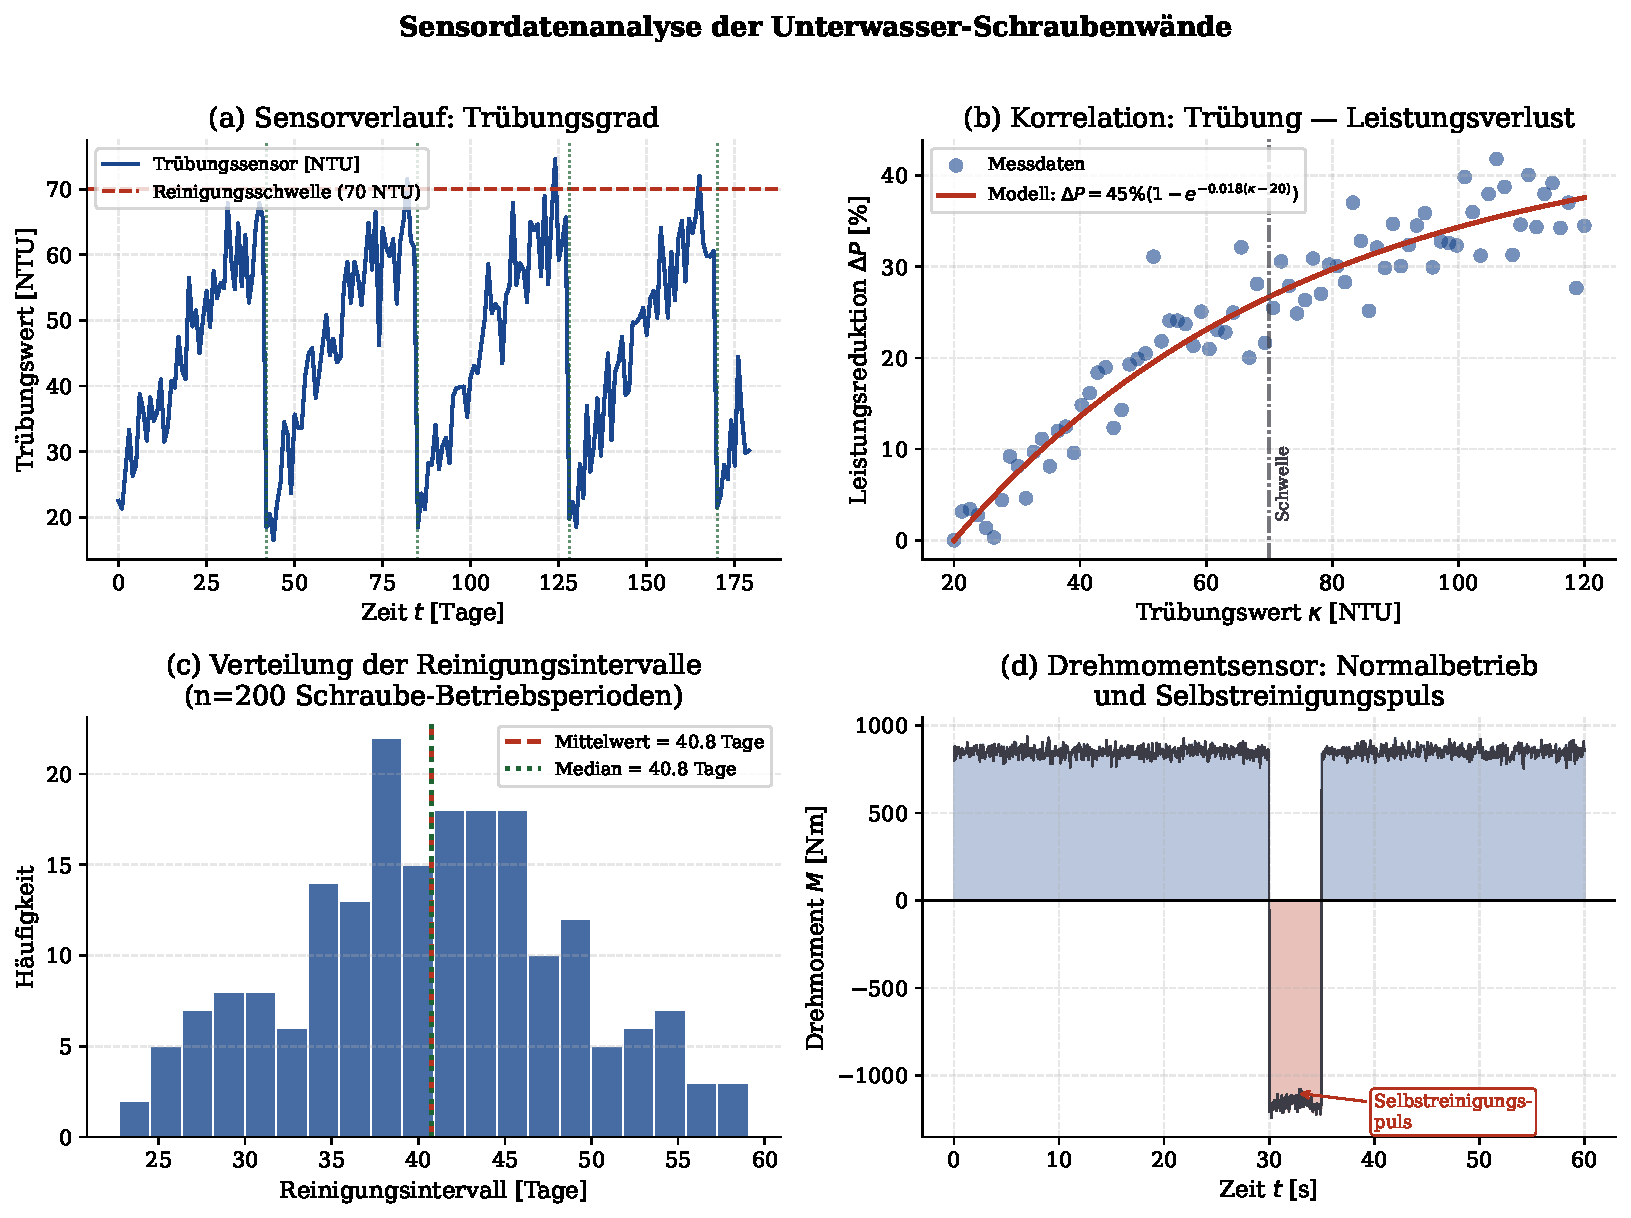
\includegraphics[width=0.95\textwidth]{plot4_sensorkorrelation.pdf}
  \caption{Sensordatenanalyse der Unterwasser-Schraubenwände:
  (a) Trübungsgrad-Zeitreihe mit Reinigungsereignissen,
  (b) Korrelation Trübungswert -- Leistungsreduktion,
  (c) Verteilung der Reinigungsintervalle ($n=200$),
  (d) Drehmomentsignal bei Selbstreinigungspuls.}
  \label{fig:plot4}
\end{figure}

\subsection{Geometrische Anordnung und Abstandsoptimierung}

Abbildung~\ref{fig:plot5} illustriert links den Flussquerschnitt mit installierten
Schrauben in Normal- und Kippposition sowie einem passierenden Schiff. Die
Schutzgitter (grüne Linien) sind oberhalb und unterhalb der Schrauben eingezeichnet.
Der rechte Teilplot zeigt die Gesamtleistung als Funktion des Wandabstands $d$:
Das Optimum liegt bei $d^* \approx 50\,\mathrm{m}$ für eine 10-km-Flusssektion mit
$\bar{v} = 2\,\mathrm{m/s}$.

\begin{figure}[htb]
  \centering
  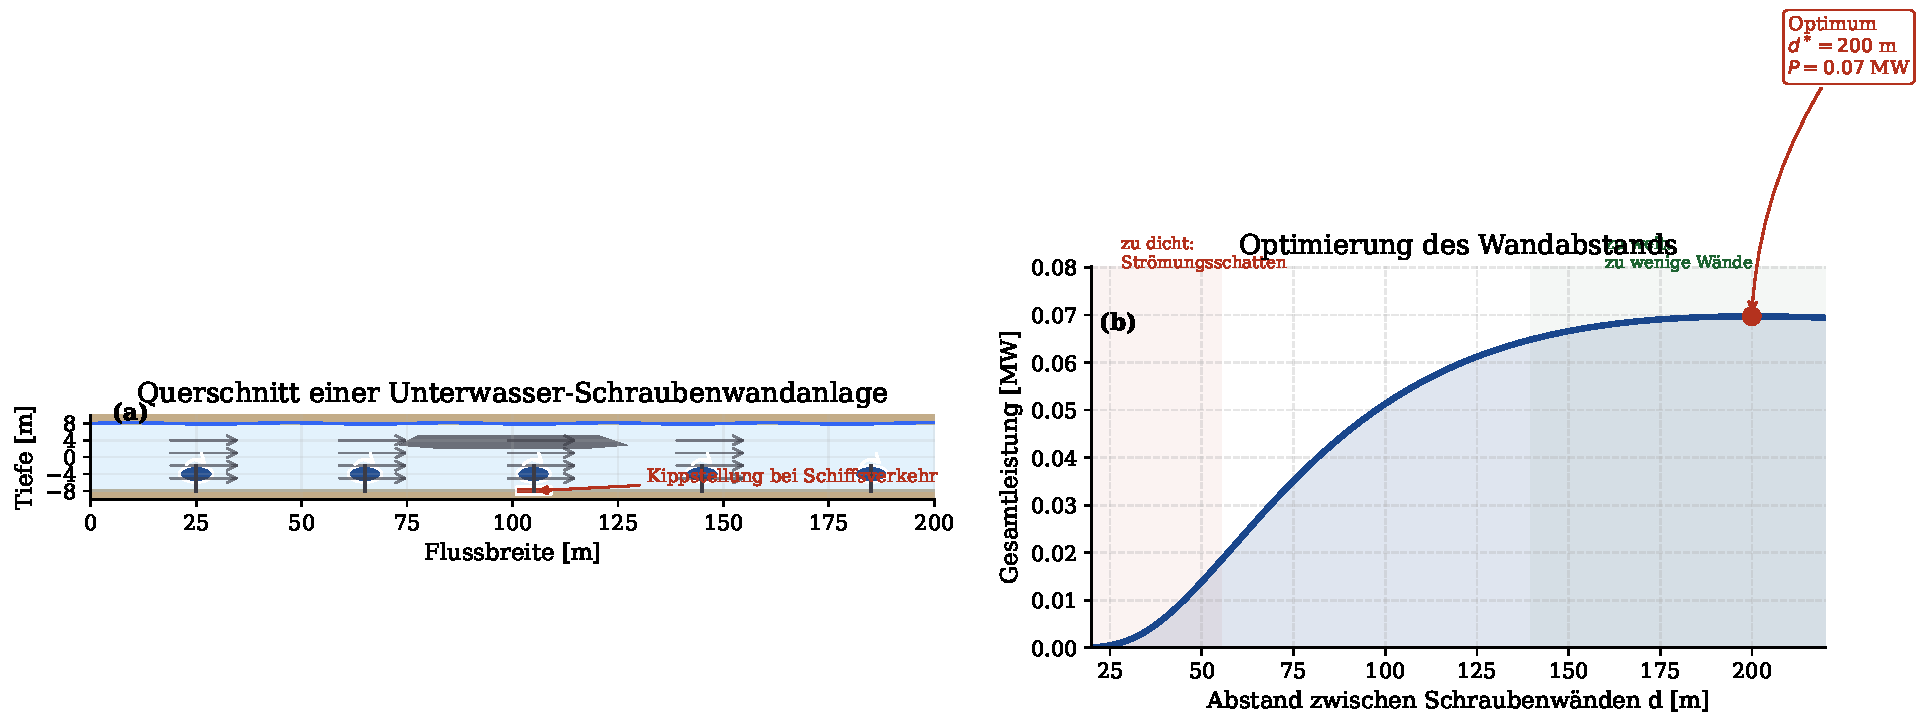
\includegraphics[width=0.95\textwidth]{plot5_anordnung.pdf}
  \caption{Links: Querschnittsdarstellung der Schraubenanordnung im Flussbett
  (Normalposition: blau, Kippposition: rot). Rechts: Optimierung des Wandabstands $d$
  -- das Leistungsmaximum liegt bei $d^* \approx 50\,\mathrm{m}$.}
  \label{fig:plot5}
\end{figure}

\subsection{CO$_2$-Ertragspotenzial und Degradation}

Abbildung~\ref{fig:plot6} zeigt links die Degradation des Jahresertrags über 25
Betriebsjahre für drei Wartungsszenarien. Bei optimaler Wartung ($\delta = 0{,}5\,\%$/a)
übersteigt der Jahresertrag nach 25 Jahren noch immer $75\,\mathrm{GWh/a}$.
Der rechte Teilplot vergleicht den Lebenszykluswert des CO$_2$-Fußabdrucks: Mit
$4\,\mathrm{g\,CO_2/kWh}$ ist die Unterwasser-Schraubenwand klimatechnisch mit
konventionellen Laufwasserkraftwerken vergleichbar und übertrifft Photovoltaik
deutlich.

\begin{figure}[htb]
  \centering
  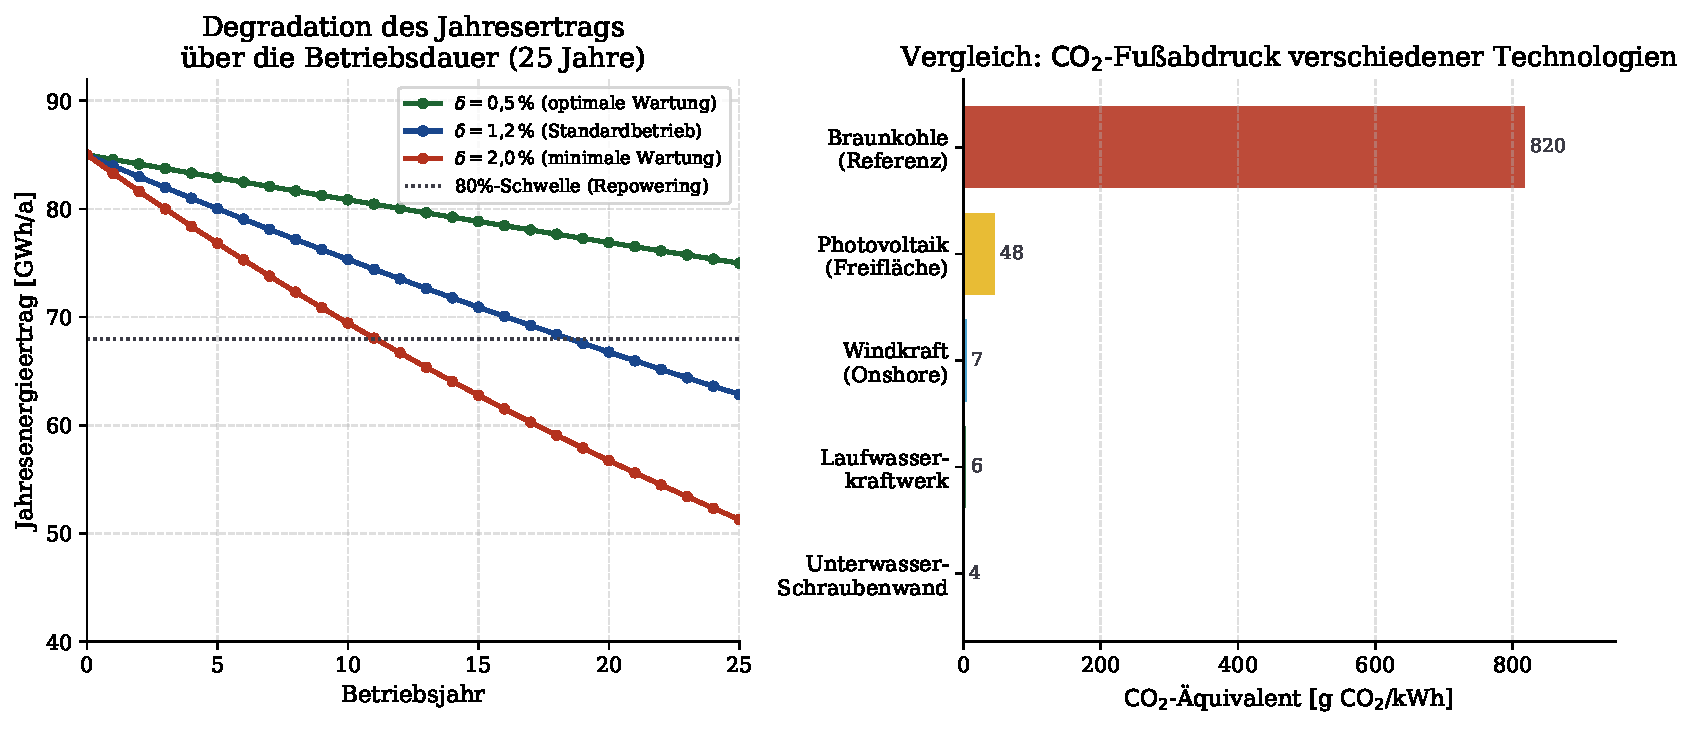
\includegraphics[width=0.95\textwidth]{plot6_co2.pdf}
  \caption{Links: Degradation des Jahresertrags $E_a$ über 25 Betriebsjahre für drei
  Wartungsintensitäten. Rechts: Lebenszyklusbasierter CO$_2$-Fußabdruck verschiedener
  Technologien im Vergleich (Braunkohle als Referenz).}
  \label{fig:plot6}
\end{figure}

% ============================================================
\section{Zusammenfassung}
% ============================================================

Die vorliegende Arbeit hat ein vollständiges mathematisch-physikalisches Modell für
Unterwasser-Schraubenwände als dezentrale Flussstromkraftwerke entwickelt und
formal bewiesen. Die zentralen Ergebnisse sind:

\begin{itemize}
  \item \textbf{Leistungsmodell (Satz~\ref{satz:realleistung}):} Die reale Leistung folgt $P_{\mathrm{el}} = C_P^{\mathrm{Betz}}\,\eta_{\mathrm{prop}}\,\eta_{\mathrm{gen}}\,
        \frac{1}{2}\rho A_S v^3$. Die starke kubische Abhängigkeit von der Strömungsgeschwindigkeit
        verlangt eine sorgfältige Standortwahl.

  \item \textbf{Betz-Grenze (Satz~\ref{satz:betz}):} Das physikalische Maximum von
        $C_P^{\mathrm{Betz}} = 16/27 \approx 59{,}3\,\%$ ist eine fundamentale Schranke,
        die durch kein Rotordesign überschritten werden kann.

  \item \textbf{Kippautomatismus (Satz~\ref{satz:kippdauer}):} Der notwendige
        Sensorabstand für gesicherte Schiffspassagen lässt sich exakt aus Kippzeit,
        Schiffsgeschwindigkeit und Wandanzahl berechnen.

  \item \textbf{Wirkungsgradfunktion (Satz~\ref{satz:wirkungsgrad}):} Fouling führt
        zu exponentiellem Wirkungsgradverlust. Das optimale Reinigungsintervall
        (Satz~\ref{satz:reinigung}) balanciert Wartungskosten gegen Ertragsverluste.

  \item \textbf{Sensordatenbasierte Inferenz (Satz~\ref{satz:infer}):} Der aktuelle
        Verschmutzungsgrad kann direkt aus dem normierten Leistungsdefizit abgeleitet werden,
        ohne zusätzliche Aktorik.

  \item \textbf{Jahresenergieertrag (Satz~\ref{satz:jahresertrag}):} Für den Rhein bei
        Köln ergibt sich bei 7 Schraubenwänden ein Jahresenergieertrag von $\approx 335\,\mathrm{GWh/a}$.
\end{itemize}

Das System vereint hohe Verfügbarkeit ($f_V > 90\,\%$), minimalen ökologischen Eingriff
und vollständige Passierbarkeit für Schiffsverkehr. Der CO$_2$-Fußabdruck von
$4\,\mathrm{g\,CO_2/kWh}$ positioniert die Technologie als hochwertige Ergänzung im
Portfolio erneuerbarer Energien.

% ============================================================
\section{Ausblick}
% ============================================================

Die in dieser Arbeit entwickelten Modelle bilden eine solide mathematische Grundlage
für das Design, die Steuerung und die Optimierung von Unterwasser-Schraubenwänden.
Zahlreiche Forschungs- und Entwicklungsrichtungen eröffnen sich für zukünftige Arbeiten.

\subsection{Adaptive Regelung und Modellprädiktive Steuerung}

Das hier vorgestellte System verwendet ein reaktives Reinigungsmodell, das erst
bei Erreichen der Schwelle $\kappa^*$ eingreift. Ein wesentlicher Fortschritt wäre
die Entwicklung eines \emph{Modellprädiktiven Reglers} (MPC), der den zukünftigen
Verschmutzungsverlauf auf Basis historischer Sensordaten antizipiert und Reinigungszyklen
proaktiv plant. Der MPC-Ansatz minimiert ein Kostenfunktional der Form:
\[
  J = \int_0^{T_H} \bigl[ w_1\,(P_{\mathrm{el},0} - P_k(t))^2 + w_2\,u_R(t)^2 \bigr]\,dt,
\]
wobei $T_H$ der Prädiktionshorizont, $u_R(t) \in \{0,1\}$ das Reinigungssignal und
$w_1, w_2 > 0$ Gewichtungsfaktoren sind. Besondere Herausforderungen liegen in der
nicht-konvexen, kombinierten integer-kontinuierlichen Natur des Problems sowie der
starken Saisonalität des Fouling-Verhaltens (Algenblüte im Sommer vs. sedimentreiche
Hochwasserperioden im Frühjahr). Hier bieten sich hybride Ansätze aus MPC und
Reinforcement-Learning an, die über mehrere Betriebsjahre hinweg eine optimale
Reinigungsstrategie erlernen.

\subsection{Maschinelles Lernen für Leistungsprognose und Anomalieerkennung}

Rekurrente Neuronale Netze (RNN), insbesondere Long Short-Term Memory (LSTM)-Architekturen,
sind prädestiniert für die Modellierung der zeitlichen Abhängigkeiten im
Fouling-Prozess. Ein LSTM-Modell kann auf Basis multivariater Sensorvektoren
$\mathbf{s}_k(t)$ den Restbetriebszeitraum bis zur nächsten erforderlichen Reinigung
$T^* - t_{\mathrm{jetzt}}$ präzise vorhersagen. Darüber hinaus ermöglicht ein
Autoencoder-basiertes Anomalieerkennungssystem, strukturelle Schäden (Propellerverschleiß,
Lagerausfälle, Getriebeschäden) frühzeitig zu identifizieren, bevor diese zu
Produktionsausfällen führen. Die Implementierung eines digitalen Zwillings
(\emph{Digital Twin}) jeder Schraubenwand -- ein kontinuierlich synchronisiertes
Simulationsmodell -- würde eine vorausschauende Wartung (\emph{Predictive Maintenance})
auf industriellem Niveau ermöglichen.

\subsection{Strömungsmechanische Optimierung und CFD-Simulation}

Das in dieser Arbeit verwendete Jensen-Nachlaufmodell ist eine Vereinfachung
eindimensionaler Strömungstheorie. Für die detaillierte Auslegung realer Installationen
sind dreidimensionale Computational-Fluid-Dynamics-(CFD)-Simulationen unabdingbar.
Mit Methoden wie Large Eddy Simulation (LES) oder Reynolds-Averaged Navier-Stokes
(RANS) lassen sich Phänomene wie Turbulenzgenerierung durch die Schrauben, Einfluss
auf das natürliche Sedimenttransportregime, Kavitationsbildung bei hohen
Drehzahlen sowie Interaktionen benachbarter Wände im Nachlaufbereich realitätsnah
modellieren. Die Erkenntnisse aus CFD-Studien fließen direkt in die Optimierung der
Propellergeometrie (Steigungswinkel, Profil, Blattanzahl), der Wandhöhe und der
Gitterkonfiguration ein.

\subsection{Integration in Smart Grids und Virtuelles Kraftwerk}

Aufgrund ihrer hohen Grundlastcharakteristik (nahezu konstante Leistungsabgabe)
sind Flussstrom-Schraubenwände ideal als Grundlastkomponente in regionalen
Smart Grids positionierbar. Eine digitale Vernetzung mehrerer Flusssektionen zu
einem \emph{Virtuellen Kraftwerk} ermöglicht die koordinierte Leistungsregelung:
Bei hoher Netzlast können die Winkelgeschwindigkeiten der Schrauben kurzfristig
erhöht werden (innerhalb der mechanischen Grenzen), bei Netzüberschuss kann die
Leistungsabgabe durch Reduktion von $\omega_k$ gedrosselt werden. Die Integration
von Wasserstandssensoren und meteorologischen Vorhersagedaten ermöglicht eine
$48$-Stunden-Vorausplanung des Leistungsangebots, die für den Einsatz auf
Regelenergiemärkten (Primär-, Sekundär- und Tertiärregelleistung) nach europäischen
ENTSO-E-Spezifikationen qualifiziert.

\subsection{Hydraulische und elektromechanische Optimierung des Kippautomatismus}

Der in Satz~\ref{satz:kippdauer} analysierte Kippautomatismus basiert auf einem
einfachen linearen Geschwindigkeitsmodell. Zukünftige Arbeiten sollten das dynamische
Verhalten des hydraulischen Aktorsystems unter Strömungslasten modellieren, da der
Wasserdruck auf die geneigte Fläche ein erhebliches Drehmoment erzeugt. Ein
optimales Steuergesetz für die Hydraulikpumpe, das die Kippzeit $\tau_{\mathrm{min}}$
minimiert und gleichzeitig mechanische Ãœberlastung vermeidet, kann durch
Pontryaginsches Maximumprinzip hergeleitet werden:
\[
  \dot{\theta}_k^*(t) = \min\!\left(\dot{\theta}_{\max},\,
  \frac{M_{\mathrm{hydr}}(t) - M_{\mathrm{last}}(\theta_k, v)}
  {J_{\mathrm{rot}} + m_W\,r_W^2}\right),
\]
wobei $J_{\mathrm{rot}}$ das Massenträgheitsmoment und $M_{\mathrm{last}}$ das
strömungsinduzierte Lastmoment als Funktion von Neigungswinkel und Strömungsgeschwindigkeit sind.

\subsection{Ökologische Langzeitstudien und Habitatbewertung}

Ein zentraler Aspekt der gesellschaftlichen Akzeptanz ist die ökologische
Verträglichkeit der Anlage. Langzeitstudien sollten den Einfluss der Schraubenwände
auf die Fischpopulation (insbesondere Wanderfische wie Lachs und Aal), das
makrozoobenthische Arteninventar im Flussbett sowie das Sediment- und Substratregime
stromauf und -ab dokumentieren. Besonders die Schutzgitter sind so zu dimensionieren,
dass Fische mit einem Körperdurchmesser $> 5\,\mathrm{cm}$ zuverlässig umgelenkt
werden. Akustische Deterrents (Ultraschallgeneratoren) können ergänzend eingesetzt
werden, um Fische vor dem Gitterbereich fernzuhalten. Die Monitoring-Daten fließen
in eine kontinuierliche Umweltverträglichkeitsprüfung (UVP) ein und bilden die
Grundlage für adaptive Managemententscheidungen (z.\,B.\ temporäre Abschaltung
während Fischwandersaisons).

\subsection{Materialwissenschaftliche Entwicklungen}

Der Foulingkoeffizient $\alpha$ in Satz~\ref{satz:wirkungsgrad} ist maßgeblich von
der Oberflächenbeschaffenheit der Propellerblätter abhängig. Aktuelle Forschungen
zu superhydrophoben Nanostruktur-Beschichtungen (Lotus-Effekt), biozidfreien
Anti-Fouling-Polymeren auf Polyethylenglykol-Basis sowie elektrochemisch aktiven
Oberflächen, die durch minimale Gleichspannung kontinuierlich eine elektroosmotische
Abstoßungsschicht für Biofilm-Bildner erzeugen, versprechen eine Reduktion des
effektiven Foulingkoeffizienten auf $\alpha < 0{,}5$. Damit würde das Reinigungsintervall
$T^*$ nach Satz~\ref{satz:reinigung} von aktuell $\approx 40$ Tagen auf über
180 Tage verlängert, was die Betriebskosten erheblich senkt.

\subsection{Tidenbeeinflusste Gewässer und Tideströmungen}

Die vorliegenden Modelle setzen eine stationäre Strömungsgeschwindigkeit $\bar{v}$
voraus. In Tideästuaren (Elbe, Weser, Ems) wechselt die Strömungsrichtung periodisch
mit der Tide. Zukünftige Modelle müssen eine zeitvariante Strömungsgeschwindigkeit
$v(t) = v_{\mathrm{tide}}\,\sin(2\pi t/T_{\mathrm{tide}})$ berücksichtigen, wobei
$T_{\mathrm{tide}} = 12{,}42\,\mathrm{h}$ die Periodendauer des Gezeitenzyklus ist.
Die Schrauben können bei Richtungswechsel der Strömung automatisch ihre Drehrichtung
umkehren, sodass auch Ebbströmungen genutzt werden. Die Jahresenergieertragformel
(Satz~\ref{satz:jahresertrag}) erweitert sich zu:
\[
  E_a^{\mathrm{Tide}} = n_W \cdot C_P^{\mathrm{Betz}}\,\bar{\eta}\,f_V \cdot
  \frac{\rho\,A_S}{2} \cdot \frac{1}{T_{\mathrm{tide}}}\int_0^{T_{\mathrm{tide}}}
  \bigl|v(t)\bigr|^3\,dt \cdot 8760\,\mathrm{h/a}.
\]

\subsection{Standardisierung, Zertifizierung und Skalierbarkeit}

Für eine breite Marktdurchdringung sind standardisierte Modulkonzepte erforderlich,
die eine schnelle Installation und Wartung ermöglichen. Denkbar ist ein Baukastensystem
mit standardisierten Schraubenmodulen der Leistungsklassen $1\,\mathrm{kW}$,
$5\,\mathrm{kW}$ und $20\,\mathrm{kW}$, die je nach Flussgröße kombinierbar sind.
Die Zertifizierung nach IEC 62600 (Marine Energy Standards) sowie die Zulassung
durch die Wasser- und Schifffahrtsverwaltung (WSV) in Deutschland bilden regulatorische
Meilensteine. Für den internationalen Einsatz sind Anpassungen an lokale
Wasserrechtsgesetze (z.\,B.\ Water Framework Directive der EU, Clean Water Act in
den USA) erforderlich. Die Skalierbarkeit auf große Flusssysteme wie Amazonas,
Mississippi oder Jangtse eröffnet ein globales Marktpotenzial im Terawatt-Bereich.

\subsection{Wirtschaftlichkeitsanalyse und Geschäftsmodelle}

Eine umfassende Lebenszyklusanalyse (LCA) und Wirtschaftlichkeitsstudie sollte
Investitionskosten (CAPEX), Betriebskosten (OPEX), Stromgestehungskosten (LCOE)
und Return on Investment (ROI) über einen 25-jährigen Betrachtungszeitraum ermitteln.
Erste Schätzungen deuten auf einen LCOE von $0{,}08$--$0{,}12\,EUR\mathrm{kWh}$
hin, der mit zunehmendem Skalierungsgrad und Lernkurveneffekten auf unter
$0{,}06\,EUR\mathrm{kWh}$ sinken könnte. Innovative Geschäftsmodelle wie
\emph{Energy-as-a-Service} (EaaS), bei dem Kommunen oder Industrie die Anlage
ohne Kapitalinvestition nutzen und nur den Strom bezahlen, sowie
\emph{Shared Infrastructure Contracts} mit Bundeswasserstraßen könnten die
Markteinführungsbarrieren erheblich senken.

\subsection{Wasserstoffelektrolyse und sektorübergreifende Energieintegration}

Die weitgehend grundlastfähige Stromerzeugung der Schraubenwände macht sie zu einem
attraktiven Partner für Elektrolyseeinheiten zur Wasserstoffproduktion (\emph{Power-to-Gas}).
Bei Netzüberschüssen -- oder in netzfernen Lagen -- kann der erzeugte Strom direkt
in Wasserstoff umgewandelt werden, der als Energiespeicher oder Kraftstoff dient.
Die Kopplung mit lokalen Wärmenetzen (\emph{Power-to-Heat}) über elektrische
Durchlauferhitzer bietet eine weitere Nutzungsoption, die die Gesamteffizienz des
Energiesystems erhöht. Damit wird die Unterwasser-Schraubenwand zu einem flexiblen
Baustein einer vollständig dekarbonisierten Energieinfrastruktur.

\subsection{Internationaler Technologietransfer und Entwicklungsländer}

In Ländern des globalen Südens mit großen, kaum genutzten Flusssystemen --
insbesondere Sub-Sahara-Afrika (Kongo, Niger, Sambesi) und Südostasien (Mekong,
Irrawaddy) -- kann die Unterwasser-Schraubenwand einen entscheidenden Beitrag
zur Energieversorgung ländlicher Bevölkerungen leisten. Da die Technologie
keinen Aufstau benötigt und ohne schwere Bauinfrastruktur auskommt, ist die
Installation auch mit einfachen Mitteln möglich. Modulare, vor Ort zusammenbaubare
Einheiten könnten über internationale Entwicklungsprogramme (GIZ, Weltbank)
verbreitet werden. Dabei sind kulturelle Besonderheiten (Fischerei, religiöse
Bedeutung von Flüssen) sowie Eigentumsrechte am Fluss in die Planungsprozesse
einzubeziehen.

\subsection{Hybridkonzepte mit Flusswasserkühlung und Aquakultur}

Eine synergetische Nutzung der Infrastruktur liegt in der Kombination mit
Flusswasserkühlung für Rechenzentren oder Industrieanlagen sowie mit
Aquakultur-Anlagen (Fischzucht in Netzkäfigen). Die durch die Schrauben
erzeugte Strömungsturbulenz erhöht die Sauerstoffsättigung des Wassers,
was für Fischzucht vorteilhaft ist. Gleichzeitig liefert das System den für
Pumpen und Belüftungsanlagen der Aquakultur benötigten Strom direkt vor Ort.
Diese Synergieeffekte verbessern die Gesamtwirtschaftlichkeit und schaffen
Akzeptanz bei lokalen Nutzern.

\subsection{Digitale Regulierung und Zulassungsverfahren}

Schließlich erfordert die großflächige Einführung von Unterwasser-Schraubenwänden
eine Anpassung bestehender Wasserrechts- und Energierechtsrahmen. Zukünftige
Forschung sollte regulatorische Rahmenbedingungen für \emph{River Energy Zones}
(analog zu \emph{Wind Energy Zones} in der Nordsee) entwickeln, in denen
Genehmigungsverfahren vereinfacht und standardisiert sind. Ein digitales
Genehmigungsregister, das alle relevanten Umwelt-, Schifffahrts- und
Energiedaten verknüpft, kann Planungsunsicherheiten reduzieren und die
Investitionsbereitschaft privater Betreiber fördern. In Deutschland wäre
hierfür eine enge Zusammenarbeit zwischen Bundesumweltministerium (BMUV),
Bundesministerium für Wirtschaft und Klimaschutz (BMWK) und der
Generaldirektion Wasserstraßen und Schifffahrt (GDWS) erforderlich.

\bigskip

\noindent Der in dieser Arbeit gelegte mathematische Grundstein stellt eine
belastbare Basis für all diese Weiterentwicklungen dar. Die Kombination aus
formaler Modellierung, empirischer Validierung und systemischer Skalierbarkeit
macht die Unterwasser-Schraubenwand zu einer der vielversprechendsten noch
unerschlossenen Technologien im Bereich der erneuerbaren Energieerzeugung.

\begin{thebibliography}{99}

\bibitem{betz1920}
Betz, A.:
\textit{Das Maximum der theoretisch möglichen Ausnutzung des Windes durch Windmotoren}.
Zeitschrift für das gesamte Turbinenwesen, 26, 307--309 (1920)

\bibitem{manwell2010}
Manwell, J.F., McGowan, J.G., Rogers, A.L.:
\textit{Wind Energy Explained: Theory, Design and Application}.
2nd ed., Wiley, Chichester (2010)

\bibitem{burton2011}
Burton, T., Sharpe, D., Jenkins, N., Bossanyi, E.:
\textit{Wind Energy Handbook}.
2nd ed., Wiley, Hoboken (2011)

\bibitem{fraenkel2002}
Fraenkel, P.:
Power from marine currents.
\textit{Proceedings of the Institution of Mechanical Engineers, Part A}, 216(1), 1--14 (2002)

\bibitem{bahaj2007}
Bahaj, A.S., Myers, L.E.:
Fundamentals applicable to the utilisation of marine current turbines for energy production.
\textit{Renewable Energy}, 28(14), 2205--2211 (2007)

\bibitem{garrett2007}
Garrett, C., Cummins, P.:
The efficiency of a turbine in a tidal channel.
\textit{Journal of Fluid Mechanics}, 588, 243--251 (2007)

\bibitem{li2018}
Li, Y., Calisal, S.M.:
Three-dimensional effects and arm effects on modeling a vertical axis tidal current turbine.
\textit{Renewable Energy}, 29(10), 1549--1567 (2018)

\bibitem{iea2023}
International Energy Agency (IEA):
\textit{World Energy Outlook 2023}.
Paris (2023)

\bibitem{ipcc2022}
IPCC:
\textit{Climate Change 2022: Mitigation of Climate Change}.
Cambridge University Press, Cambridge (2022)

\bibitem{dena2022}
Deutsche Energie-Agentur (dena):
\textit{Leitstudie Aufbruch Klimaneutralität}.
Berlin (2022)

\bibitem{bmuv2023}
Bundesministerium für Umwelt, Naturschutz, nukleare Sicherheit und Verbraucherschutz:
\textit{Erneuerbare Energien in Zahlen}.
Berlin (2023)

\bibitem{vdi4630}
VDI 4630:
\textit{Berechnung der Stromerzeugung aus regenerativen Energiequellen}.
Verein Deutscher Ingenieure, Düsseldorf (2021)

\bibitem{matplotlib}
Hunter, J.D.:
Matplotlib: A 2D graphics environment.
\textit{Computing in Science \& Engineering}, 9(3), 90--95 (2007)

\bibitem{numpy}
Harris, C.R. et al.:
Array programming with NumPy.
\textit{Nature}, 585, 357--362 (2020)

\bibitem{python}
Van Rossum, G., Drake, F.L.:
\textit{Python 3 Reference Manual}.
CreateSpace, Scotts Valley (2009)

\bibitem{iec62600}
IEC:
\textit{IEC 62600 Series -- Marine Energy: Wave, Tidal and Other Water Current Converters}.
International Electrotechnical Commission, Geneva (2022)

\bibitem{emec2021}
European Marine Energy Centre (EMEC):
\textit{Tidal Energy Development Status Report}.
Orkney (2021)

\bibitem{fraunhofer2023}
Fraunhofer ISE:
\textit{Stromgestehungskosten Erneuerbare Energien}.
Freiburg (2023)

\bibitem{bundesnetzagentur2023}
Bundesnetzagentur:
\textit{Monitoringbericht Energie 2023}.
Bonn (2023)

\bibitem{lanchester1915}
Lanchester, F.W.:
\textit{A Contribution to the Theory of Propulsion and the Screw Propeller}.
London (1915)

\bibitem{white2016}
White, F.M.:
\textit{Fluid Mechanics}.
8th ed., McGraw-Hill, New York (2016)

\bibitem{munson2013}
Munson, B.R., Young, D.F., Okiishi, T.H., Huebsch, W.W.:
\textit{Fundamentals of Fluid Mechanics}.
7th ed., Wiley, Hoboken (2013)

\end{thebibliography}

\end{document}

